% Options for packages loaded elsewhere
\PassOptionsToPackage{unicode}{hyperref}
\PassOptionsToPackage{hyphens}{url}
%
\documentclass[
]{article}
\usepackage{lmodern}
\usepackage{amssymb,amsmath}
\usepackage{ifxetex,ifluatex}
\ifnum 0\ifxetex 1\fi\ifluatex 1\fi=0 % if pdftex
  \usepackage[T1]{fontenc}
  \usepackage[utf8]{inputenc}
  \usepackage{textcomp} % provide euro and other symbols
\else % if luatex or xetex
  \usepackage{unicode-math}
  \defaultfontfeatures{Scale=MatchLowercase}
  \defaultfontfeatures[\rmfamily]{Ligatures=TeX,Scale=1}
\fi
% Use upquote if available, for straight quotes in verbatim environments
\IfFileExists{upquote.sty}{\usepackage{upquote}}{}
\IfFileExists{microtype.sty}{% use microtype if available
  \usepackage[]{microtype}
  \UseMicrotypeSet[protrusion]{basicmath} % disable protrusion for tt fonts
}{}
\makeatletter
\@ifundefined{KOMAClassName}{% if non-KOMA class
  \IfFileExists{parskip.sty}{%
    \usepackage{parskip}
  }{% else
    \setlength{\parindent}{0pt}
    \setlength{\parskip}{6pt plus 2pt minus 1pt}}
}{% if KOMA class
  \KOMAoptions{parskip=half}}
\makeatother
\usepackage{xcolor}
\IfFileExists{xurl.sty}{\usepackage{xurl}}{} % add URL line breaks if available
\IfFileExists{bookmark.sty}{\usepackage{bookmark}}{\usepackage{hyperref}}
\hypersetup{
  hidelinks,
  pdfcreator={LaTeX via pandoc}}
\urlstyle{same} % disable monospaced font for URLs
\usepackage{graphicx}
\makeatletter
\def\maxwidth{\ifdim\Gin@nat@width>\linewidth\linewidth\else\Gin@nat@width\fi}
\def\maxheight{\ifdim\Gin@nat@height>\textheight\textheight\else\Gin@nat@height\fi}
\makeatother
% Scale images if necessary, so that they will not overflow the page
% margins by default, and it is still possible to overwrite the defaults
% using explicit options in \includegraphics[width, height, ...]{}
\setkeys{Gin}{width=\maxwidth,height=\maxheight,keepaspectratio}
% Set default figure placement to htbp
\makeatletter
\def\fps@figure{htbp}
\makeatother
\setlength{\emergencystretch}{3em} % prevent overfull lines
\providecommand{\tightlist}{%
  \setlength{\itemsep}{0pt}\setlength{\parskip}{0pt}}
\setcounter{secnumdepth}{-\maxdimen} % remove section numbering

\author{}
\date{}

\begin{document}

\hypertarget{header-n1582}{%
\section{ENSOR}\label{header-n1582}}

Ensor is a python program with advanced partitioning algorithms for
optimizing Quantum calculation for large molecules.

\begin{quote}
If one can divide a species of interest into fragments, employ some
level of ab-initio QM to calculate the wave function, energy, and
properties of each fragment, and then combine the results from the
fragment calculations to predict the same properties for the whole, the
possibility exists that the accuracy of the outcome can approach that
which would be obtained from a full non fragmented calculation.
\end{quote}

\hypertarget{header-n1587}{%
\subsubsection{Table of Contents}\label{header-n1587}}

\begin{itemize}
\item
  \protect\hyperlink{partitioning-algorithm}{Partitioning Algorithm}

  \begin{itemize}
  \item
    \protect\hyperlink{building-connectivity-of-molecule}{Building
    Connectivity of Molecule}
  \item
    \protect\hyperlink{spectral-graph-partitioning}{Spectral Graph
    Partitioning}
  \item
    \protect\hyperlink{header-n1629}{Algorithm}
  \item
    \protect\hyperlink{overlaps-selection}{Overlaps Selection}
  \item
    \protect\hyperlink{adding-hydrogen}{Adding Hydrogen}
  \end{itemize}
\end{itemize}

\hypertarget{header-n1590}{%
\paragraph{Partitioning Algorithm}\label{header-n1590}}

\hypertarget{header-n1604}{%
\subparagraph{Building Connectivity of Molecule}\label{header-n1604}}

We build Connectivity by assigning weight to the Matrix \(C_{n,n}\)
representing connectedness between atoms as.

\begin{itemize}
\item
  \(w_{ij}=w_{0}^{\bigg(1-\dfrac{r_{ij}^2}{r^2_0}\bigg)}\) where \(r_0\)
  is single-bond length between atoms.

  \begin{figure}
  \centering
  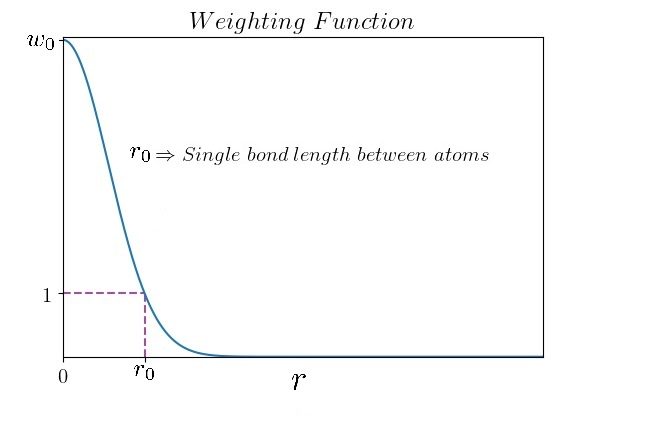
\includegraphics{C:/Users/Healer/Project/ensor/image/gausconw.jpeg}
  \caption{}
  \end{figure}
\end{itemize}

So, weighted connectivity \(C\) is \\
\(C_{i,j}=w_{ij}\)

\hypertarget{header-n1611}{%
\subparagraph{Spectral Graph Partitioning}\label{header-n1611}}

We define Laplacian \(L\) as

\begin{itemize}
\item
  \(L=D-C\) where \(D_{n,n}=diag(d_1,d_2,..,d_n)\) with
  \(d_i=\sum_{j=1}^{n} C_{i,j}=\sum_{j=1}^{n} w_{ij}\)

  \begin{quote}
  The Laplacian of any graph \(G\) have a balanced division knowledge,
  but the \(G\) must be a one connected component. Otherwise a balanced
  division does not occur.
  \end{quote}
\end{itemize}

After normalization, we get,

\begin{equation}
L_{i,j}=\begin{cases}
       \text{1,} &\quad\text{if i=j}\\
       -\dfrac{w_{ij}}{\sqrt{d_id_j}}\text{,} &\quad\text{if i$\neq$j}\\
     \end{cases}
\end{equation}

Because \(L\) is a symmetric matrix, its eigenvalues are real, and its
eigenvectors are orthogonal to each other. Calculating eigenvalues and
eigenvector using \(Lv={\lambda} v\), the eigenvector corresponding to
the second smallest eigenvalue(\(\lambda_{2}\)) of L(G) is known as the
Fiedler vector(\(f_{2}\)).

we can partition the molecule in two parts using these eigenvectors.

\begin{quote}
if \(f^n_2>median(f_2)\) than node n is in \(part_A\) else in \(part_B\)
\end{quote}

Partition of 804 atom nanotube using eigenvector corresponding to first,
second, third, fourth eigen values.

\begin{figure}
\centering
\includegraphics{C:/Users/Healer/Project/ensor/image/evalnano.png}
\caption{}
\end{figure}

Partition for different molecules(each atom's color represent value of
that atom corresponding to second eigen vector)

\begin{figure}
\centering
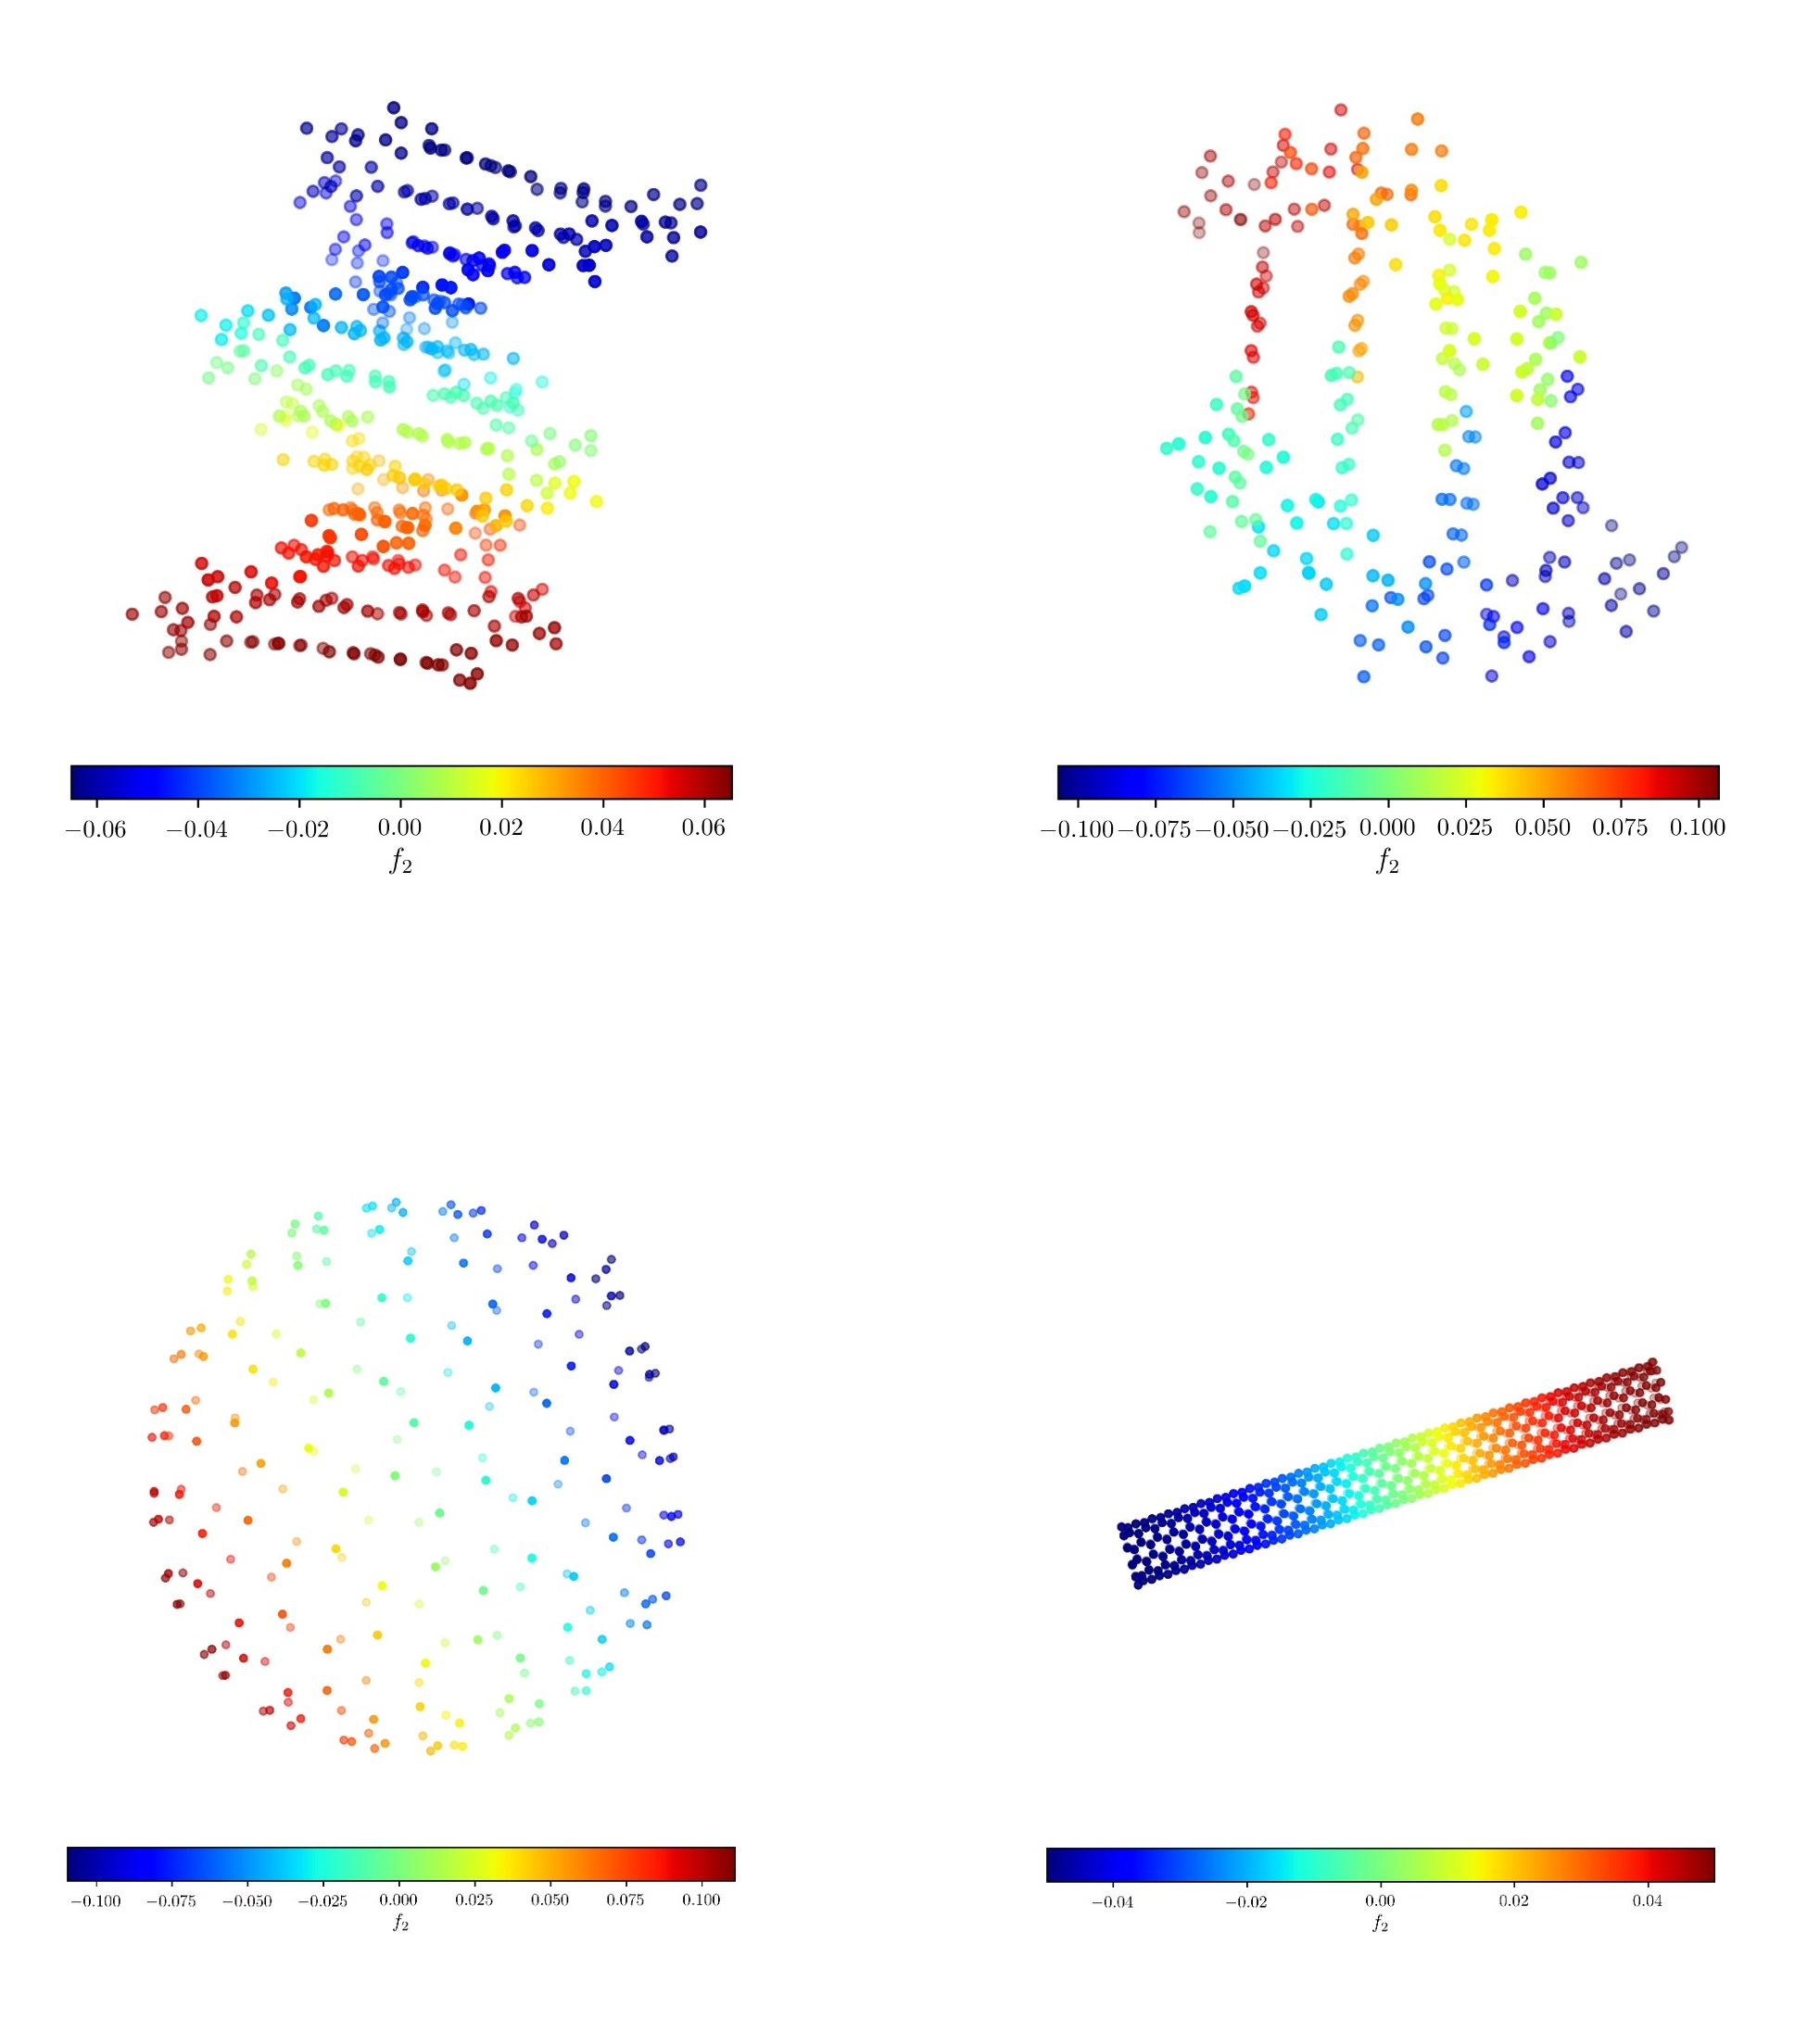
\includegraphics{C:/Users/Healer/Project/ensor/image/mols.jpeg}
\caption{}
\end{figure}

\hypertarget{header-n1629}{%
\subparagraph{\texorpdfstring{Algorithm
}{Algorithm }}\label{header-n1629}}

\begin{figure}
\centering
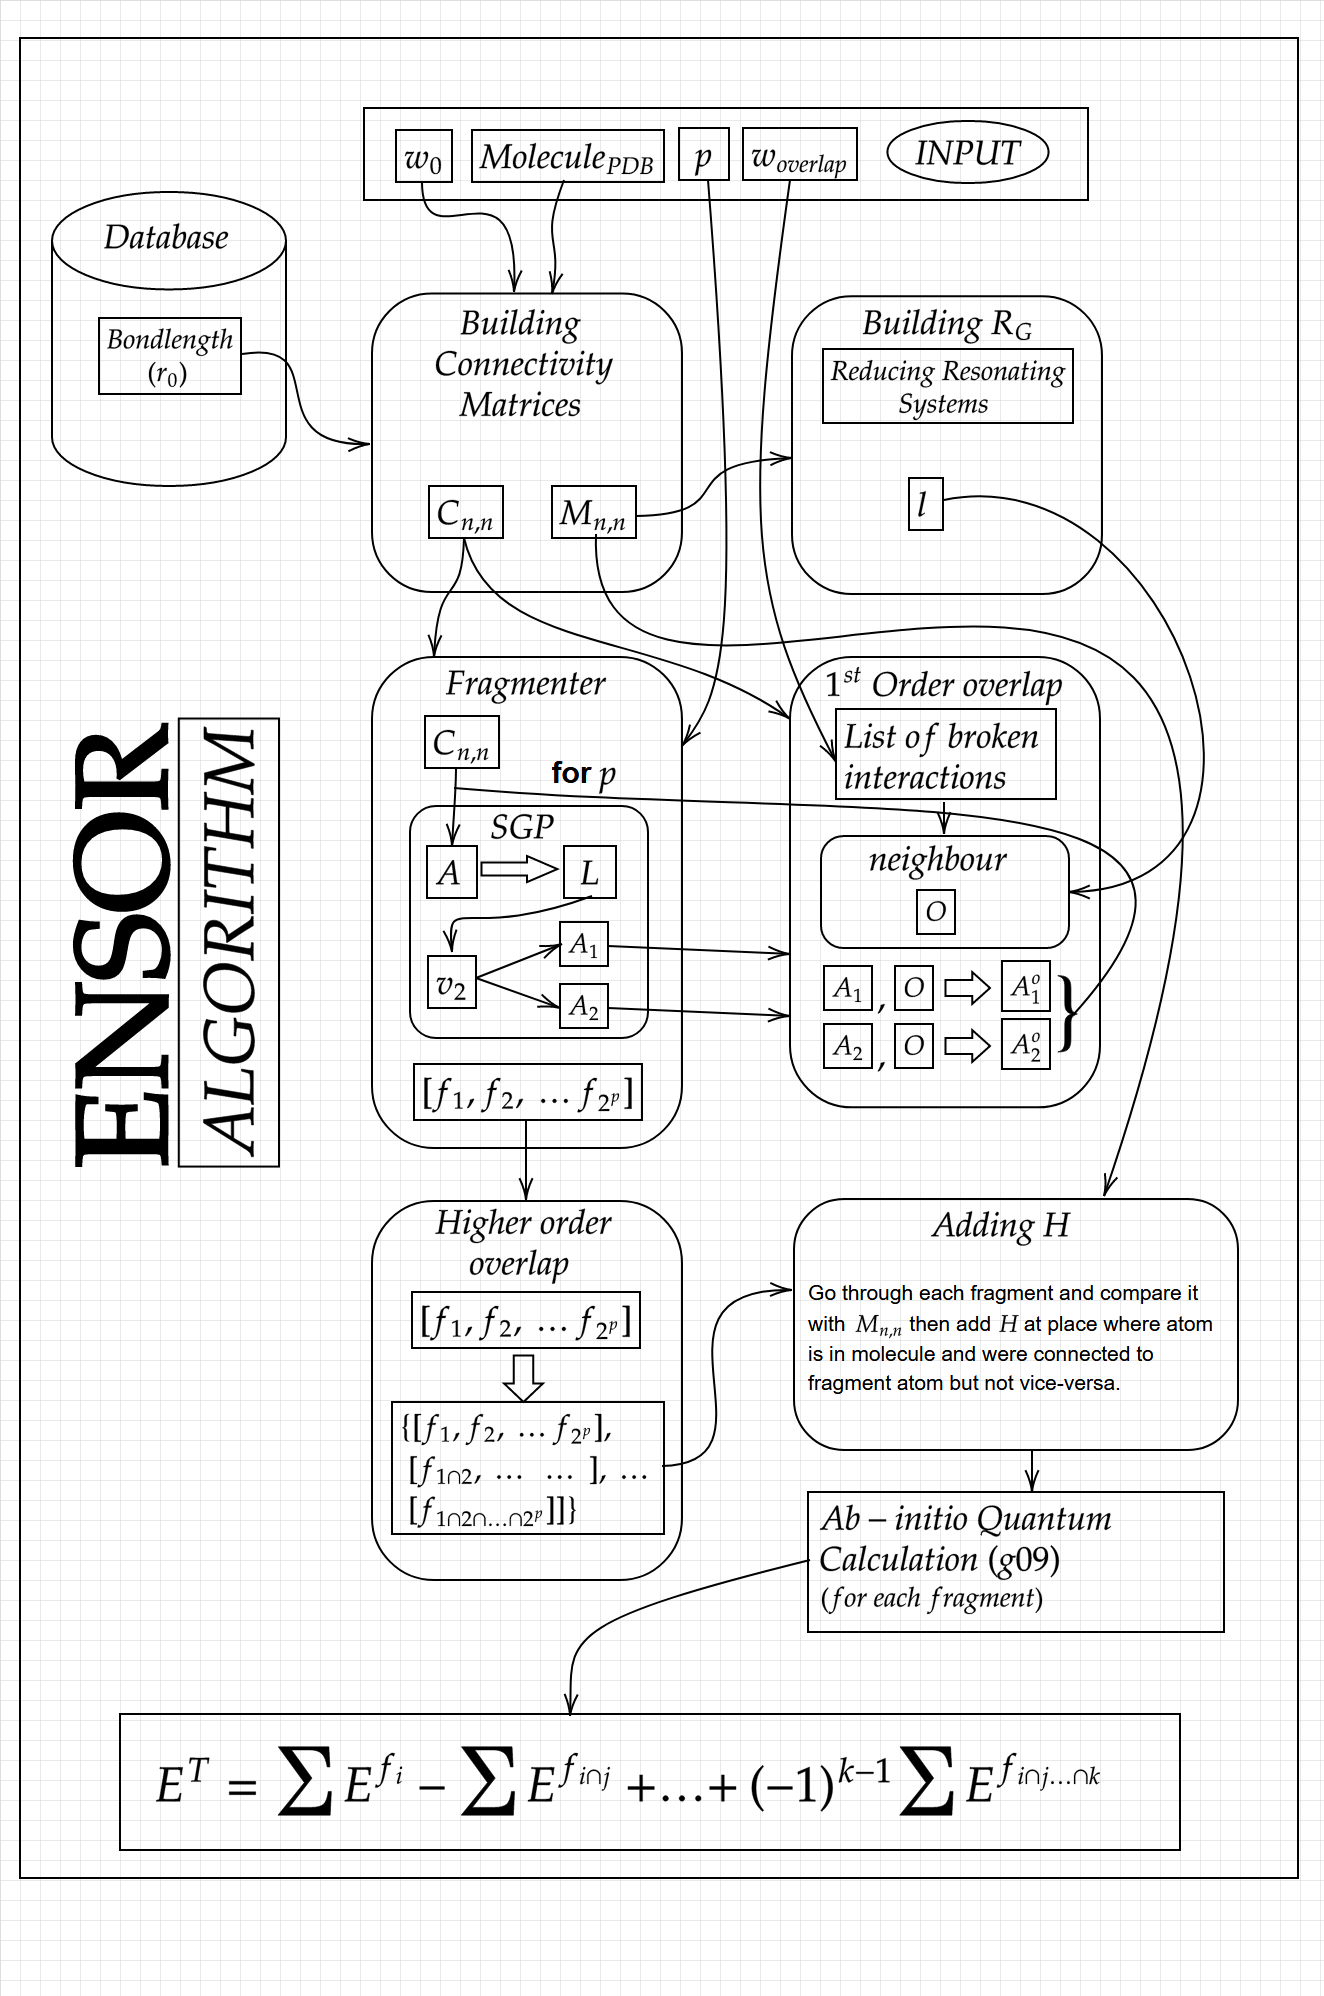
\includegraphics{C:/Users/Healer/Project/ensor/image/algorithm.png}
\caption{}
\end{figure}

\hypertarget{header-n1631}{%
\subparagraph{Overlap Selection}\label{header-n1631}}

After splitting the molecule in two parts, we calculate overlap extend
using those atom with some cut-off weightage, which were connected in
main molecule but not in fragments.

we define \(w_{overlap}\) as the minimum cut-off weight between atom ,to
start adding those atom in overlap.

We have main molecule as \(G\) but for selecting neighbor and overlap,
we use reduced \(R_G\) graph to crawl, as we have to cover all of that
resonating system even if we count one atom of that system in overlap.

\(G\) \(R_G\)

\begin{figure}
\centering
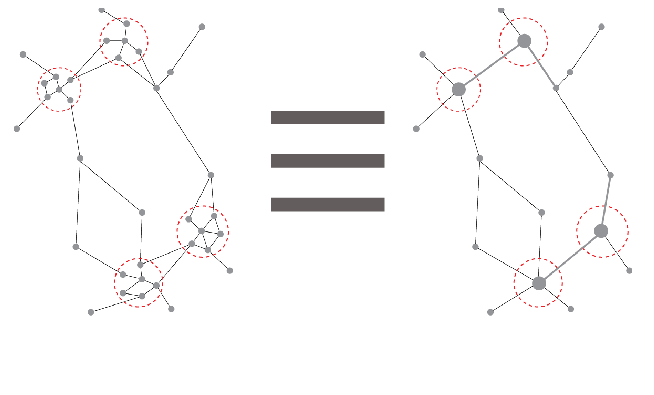
\includegraphics{C:/Users/Healer/Project/ensor/image/gred.png}
\caption{}
\end{figure}

\(R_G\) is \(G\) but with \{aromatic rings, resonating system, double
and triple bonds\} Grouped as one node.

we also defined \(Neighbor(atom,c,R_G)\) where c is the cut-off weight
over which we assume atoms are connected and are neighbor.

which returns all neighbor of the atom in \(R_G\). So, now we can go
multiple level of neighbors to extend the overlap.

\hypertarget{header-n1643}{%
\subparagraph{Adding Hydrogens}\label{header-n1643}}

After getting all fragments, we go through each one and compare them
with main Molecule then add H atoms at that place where atom is in
molecule and were connected to fragment atom but not vice-versa.

\hypertarget{header-n1645}{%
\subparagraph{Under Construction...}\label{header-n1645}}

\end{document}
